\documentclass[11pt,letterpaper,english]{article}

\usepackage[margin=1.0in]{geometry}
\usepackage{helvetica}
\usepackage{graphicx}

\newcommand{\newpar}{\vspace{10mm}\noindent}

\title{An Analysis of Monsanto's Earning Announcement}
\author{Ian Clark}
\date{}

\begin{document}
\maketitle

\section{Results of the Earnings Report Upon the Market}
The market opened with news of Monsanto's Earnings Report readily available causing a rise--a $\Delta{P_{MON}} = 1.54 $--between the dates of 31 March 2015 closing and 01 April 2015 opening--01 April being the date where the earnings report was made available. There seemed to be a fair amount of inter day volatility within MON, as it reached a high of $117.13$ and a low of $113.62$. However, Monsanto ended the day trading near its high at $116.96$. As indicated by the chart below, we can see that Monsanto's stock price was much more volatile than in the nearly two weeks prior.

\newpar
\begin{center}
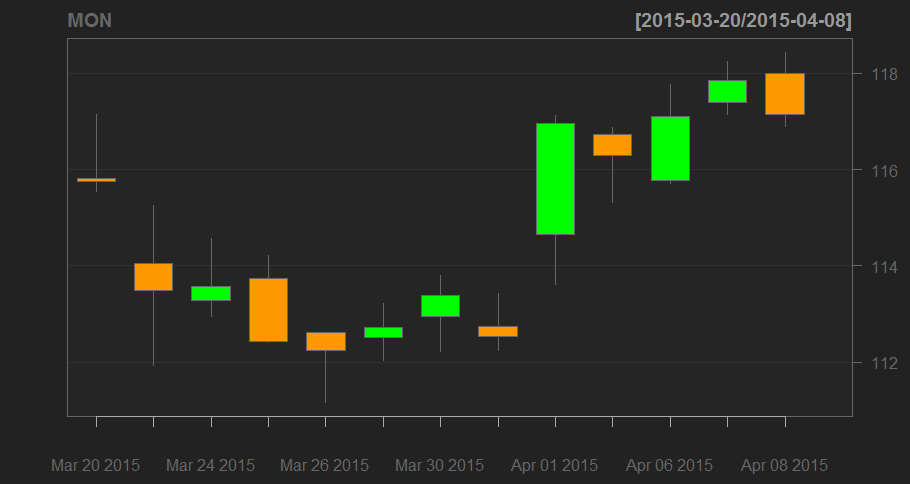
\includegraphics[scale=0.5]{Data/CandleChart.png}
\end{center}

\newpar
\subsection{Earnings per Share}
By Monsanto's estimates, their Earnings per Share ($2.92 \$ $) has remained within their estimates, but fallen over the course of the year toward the lower end of their acceptable range. A factor assumed to be heavily affecting both Monsanto and the US economy as a whole is the strengthening of the dollar in relations to other currencies--notably the Euro.

\newpar
In the second quarter of 2014, Monsanto reported an EPS of $3.15 \$ $. Therefore, Monsanto has realized a $\%\Delta{EPS} = -7$. Given that Monsanto still remains within their targeted range of EPS, this decrease, in and of itself, should not be too frightening for investors or potential investors. Although it may not be too frightening, the fact that the EPS has been decreasing for the previous two quarters indicates larger problems. As stated previously, the strengthening dollar has been causing ripples throughout the economy, Monsanto included.

\section{Growth}
While some of the more common metrics of growth may look less than promising, Monsanto has consistently been hitting milestones which will aide their future growth.

\subsection{Revenue Growth}
Monsanto announced net sales of nearly $5.2$ billion showing a decrease from net sales in the second quarter of 2014. While there may seem to be much negative news within this release, most of it appears to be noise given that both revenue growth and EPS are well within their previously established ranges.

\subsection{Margin Growth}

\newpage
\begin{thebibliography}{9}
\bibitem{Monsanto Earnings Presentation}
    Monsanto,
    \emph{$http://www.monsanto.com/investors/documents/2015/2015.04.01_mon_q2fy15_earnings.pdf$}.
\bibitem{Yahoo Finance Coverage of Report}
     Yahoo Finance,
     \emph{$http://finance.yahoo.com/news/monsanto-announces-second-quarter-financial-120000678.html$}
\end{thebibliography}

\end{document} 